\documentclass[tikz,border=4pt,11pt]{standalone}
\usepackage{amsmath}
\definecolor{ink}{RGB}{42,52,64}
\definecolor{first}{RGB}{146,79,26}

% The 15 increasing ordered trees on [4] (root 1 on top, children ordered
% left to right), grouped by child-count partition: six trees of type (3),
% eight of type (2,1) and one of type (1,1,1), matching
% L_{4,1} = 6 e_3 + 8 e_{21} + e_{111}.
% Coordinates generated by a script that enumerates the trees.

\begin{document}
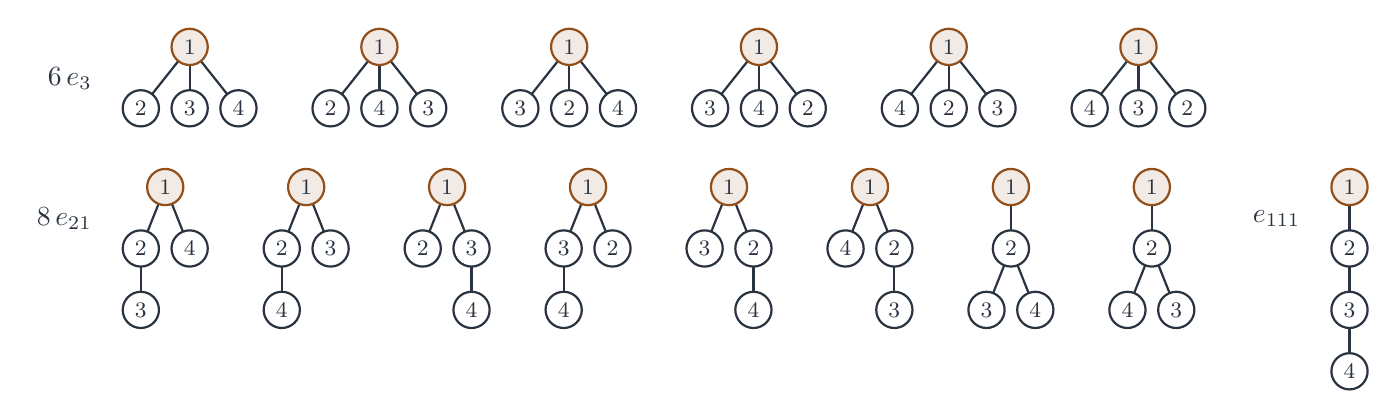
\begin{tikzpicture}[text=ink,line cap=round,
  vtx/.style={circle,draw=ink,fill=white,line width=.8pt,inner sep=0pt,
    minimum size=4.6mm,font=\footnotesize},
  root/.style={vtx,draw=first,fill=first!12}]
  % child-count partition (3,): 1(234), 1(243), 1(324), 1(342), 1(423), 1(432)
  \node[anchor=east] at (-0.500,-0.400) {$6\,e_3$};
  \draw[ink,line width=.8pt] (0.620,0.000) -- (0.000,-0.780);
  \draw[ink,line width=.8pt] (0.620,0.000) -- (0.620,-0.780);
  \draw[ink,line width=.8pt] (0.620,0.000) -- (1.240,-0.780);
  \node[root] at (0.620,0.000) {$1$};
  \node[vtx] at (0.000,-0.780) {$2$};
  \node[vtx] at (0.620,-0.780) {$3$};
  \node[vtx] at (1.240,-0.780) {$4$};
  \draw[ink,line width=.8pt] (3.030,0.000) -- (2.410,-0.780);
  \draw[ink,line width=.8pt] (3.030,0.000) -- (3.030,-0.780);
  \draw[ink,line width=.8pt] (3.030,0.000) -- (3.650,-0.780);
  \node[root] at (3.030,0.000) {$1$};
  \node[vtx] at (2.410,-0.780) {$2$};
  \node[vtx] at (3.650,-0.780) {$3$};
  \node[vtx] at (3.030,-0.780) {$4$};
  \draw[ink,line width=.8pt] (5.440,0.000) -- (4.820,-0.780);
  \draw[ink,line width=.8pt] (5.440,0.000) -- (5.440,-0.780);
  \draw[ink,line width=.8pt] (5.440,0.000) -- (6.060,-0.780);
  \node[root] at (5.440,0.000) {$1$};
  \node[vtx] at (5.440,-0.780) {$2$};
  \node[vtx] at (4.820,-0.780) {$3$};
  \node[vtx] at (6.060,-0.780) {$4$};
  \draw[ink,line width=.8pt] (7.850,0.000) -- (7.230,-0.780);
  \draw[ink,line width=.8pt] (7.850,0.000) -- (7.850,-0.780);
  \draw[ink,line width=.8pt] (7.850,0.000) -- (8.470,-0.780);
  \node[root] at (7.850,0.000) {$1$};
  \node[vtx] at (8.470,-0.780) {$2$};
  \node[vtx] at (7.230,-0.780) {$3$};
  \node[vtx] at (7.850,-0.780) {$4$};
  \draw[ink,line width=.8pt] (10.260,0.000) -- (9.640,-0.780);
  \draw[ink,line width=.8pt] (10.260,0.000) -- (10.260,-0.780);
  \draw[ink,line width=.8pt] (10.260,0.000) -- (10.880,-0.780);
  \node[root] at (10.260,0.000) {$1$};
  \node[vtx] at (10.260,-0.780) {$2$};
  \node[vtx] at (10.880,-0.780) {$3$};
  \node[vtx] at (9.640,-0.780) {$4$};
  \draw[ink,line width=.8pt] (12.670,0.000) -- (12.050,-0.780);
  \draw[ink,line width=.8pt] (12.670,0.000) -- (12.670,-0.780);
  \draw[ink,line width=.8pt] (12.670,0.000) -- (13.290,-0.780);
  \node[root] at (12.670,0.000) {$1$};
  \node[vtx] at (13.290,-0.780) {$2$};
  \node[vtx] at (12.670,-0.780) {$3$};
  \node[vtx] at (12.050,-0.780) {$4$};
  % child-count partition (2, 1): 1(2(3)4), 1(2(4)3), 1(23(4)), 1(3(4)2), 1(32(4)), 1(42(3)), 1(2(34)), 1(2(43))
  \node[anchor=east] at (-0.500,-2.180) {$8\,e_{21}$};
  \draw[ink,line width=.8pt] (0.310,-1.780) -- (0.000,-2.560);
  \draw[ink,line width=.8pt] (0.310,-1.780) -- (0.620,-2.560);
  \draw[ink,line width=.8pt] (0.000,-2.560) -- (0.000,-3.340);
  \node[root] at (0.310,-1.780) {$1$};
  \node[vtx] at (0.000,-2.560) {$2$};
  \node[vtx] at (0.000,-3.340) {$3$};
  \node[vtx] at (0.620,-2.560) {$4$};
  \draw[ink,line width=.8pt] (2.100,-1.780) -- (1.790,-2.560);
  \draw[ink,line width=.8pt] (2.100,-1.780) -- (2.410,-2.560);
  \draw[ink,line width=.8pt] (1.790,-2.560) -- (1.790,-3.340);
  \node[root] at (2.100,-1.780) {$1$};
  \node[vtx] at (1.790,-2.560) {$2$};
  \node[vtx] at (2.410,-2.560) {$3$};
  \node[vtx] at (1.790,-3.340) {$4$};
  \draw[ink,line width=.8pt] (3.890,-1.780) -- (3.580,-2.560);
  \draw[ink,line width=.8pt] (3.890,-1.780) -- (4.200,-2.560);
  \draw[ink,line width=.8pt] (4.200,-2.560) -- (4.200,-3.340);
  \node[root] at (3.890,-1.780) {$1$};
  \node[vtx] at (3.580,-2.560) {$2$};
  \node[vtx] at (4.200,-2.560) {$3$};
  \node[vtx] at (4.200,-3.340) {$4$};
  \draw[ink,line width=.8pt] (5.680,-1.780) -- (5.370,-2.560);
  \draw[ink,line width=.8pt] (5.680,-1.780) -- (5.990,-2.560);
  \draw[ink,line width=.8pt] (5.370,-2.560) -- (5.370,-3.340);
  \node[root] at (5.680,-1.780) {$1$};
  \node[vtx] at (5.990,-2.560) {$2$};
  \node[vtx] at (5.370,-2.560) {$3$};
  \node[vtx] at (5.370,-3.340) {$4$};
  \draw[ink,line width=.8pt] (7.470,-1.780) -- (7.160,-2.560);
  \draw[ink,line width=.8pt] (7.470,-1.780) -- (7.780,-2.560);
  \draw[ink,line width=.8pt] (7.780,-2.560) -- (7.780,-3.340);
  \node[root] at (7.470,-1.780) {$1$};
  \node[vtx] at (7.780,-2.560) {$2$};
  \node[vtx] at (7.160,-2.560) {$3$};
  \node[vtx] at (7.780,-3.340) {$4$};
  \draw[ink,line width=.8pt] (9.260,-1.780) -- (8.950,-2.560);
  \draw[ink,line width=.8pt] (9.260,-1.780) -- (9.570,-2.560);
  \draw[ink,line width=.8pt] (9.570,-2.560) -- (9.570,-3.340);
  \node[root] at (9.260,-1.780) {$1$};
  \node[vtx] at (9.570,-2.560) {$2$};
  \node[vtx] at (9.570,-3.340) {$3$};
  \node[vtx] at (8.950,-2.560) {$4$};
  \draw[ink,line width=.8pt] (11.050,-1.780) -- (11.050,-2.560);
  \draw[ink,line width=.8pt] (11.050,-2.560) -- (10.740,-3.340);
  \draw[ink,line width=.8pt] (11.050,-2.560) -- (11.360,-3.340);
  \node[root] at (11.050,-1.780) {$1$};
  \node[vtx] at (11.050,-2.560) {$2$};
  \node[vtx] at (10.740,-3.340) {$3$};
  \node[vtx] at (11.360,-3.340) {$4$};
  \draw[ink,line width=.8pt] (12.840,-1.780) -- (12.840,-2.560);
  \draw[ink,line width=.8pt] (12.840,-2.560) -- (12.530,-3.340);
  \draw[ink,line width=.8pt] (12.840,-2.560) -- (13.150,-3.340);
  \node[root] at (12.840,-1.780) {$1$};
  \node[vtx] at (12.840,-2.560) {$2$};
  \node[vtx] at (13.150,-3.340) {$3$};
  \node[vtx] at (12.530,-3.340) {$4$};
  % child-count partition (1, 1, 1): 1(2(3(4)))
  \node[anchor=east] at (14.850,-2.180) {$e_{111}$};
  \draw[ink,line width=.8pt] (15.350,-1.780) -- (15.350,-2.560);
  \draw[ink,line width=.8pt] (15.350,-2.560) -- (15.350,-3.340);
  \draw[ink,line width=.8pt] (15.350,-3.340) -- (15.350,-4.120);
  \node[root] at (15.350,-1.780) {$1$};
  \node[vtx] at (15.350,-2.560) {$2$};
  \node[vtx] at (15.350,-3.340) {$3$};
  \node[vtx] at (15.350,-4.120) {$4$};
\end{tikzpicture}
\end{document}
